\section{Grundlagen von Multi-Object Tracking Systemen}
Die fundamentale Aufgabe eines \gls{MOT} Systems besteht darin in einem Video mehrere Objekte zu \glsdisp{Detektion}{detektieren} und die Identitäten der Objekte über alle \gls{Frame}[s] aufrecht zu erhalten. Das Ergebnis sind die \gls{Trajektorie}[n] der Objekte \cite{CLEAR.2008, HOTA, Luo.2022}. \gls{MOT} zählt zu der Wissenschaft des maschinellen Sehens. Es ist ein recht junges Forschungsgebiet, weshalb bisher wenig verallgemeinernde Theorie existiert. Es gibt jedoch Bestrebungen grundlegende Theorie aus den zahlreichen Ansätzen in der Literatur zu extrahieren \cite{Luo.2022}. Im Fokus der Forschung liegt besonders das Tracking von Fußgängern, aufgrund von großem kommerziellen Potential. In diesem Feld ist \gls{MOT} beispielsweise anwendbar in der Überwachung, im autonomen Fahren und im Sport. Aber auch in anderen Anwendungsfeldern wir an \gls{MOT} geforscht, wie zum Beispiel am Tracking von Fahrzeugen, Partikeln, Zellen und Tieren \cite{Luo.2022, CLEAR.2008, Crocker.1996}. Die Vielzahl an Anwendungsmöglichkeiten zeigt, dass \gls{MOT} als \gls{Mid-Level Aufgabe} zu verordnen ist, auf welcher weiterreichende Anwendungen aufbauen können \cite{Luo.2022}.\par

Ein ideales \gls{MOT} System ist in der Lage zu jedem Zeitpunkt die korrekte Anzahl an Objekten zu \glsdisp{Detektion}{detektieren} und deren Positionen exakt zu bestimmen. Den Objekten wird eine Identifikationsnummer (\acrshort{ID}) zugeordnet, welche über alle Zeitpunkte hinweg konstant bleibt \cite{CLEAR.2008}. Der verbreitetste Ansatz, um diese Aufgaben zu erfüllen sind \glsdisp{Detektionsbasiertes Tracking}{detetkionsbasierte Tracking} Systeme. Diese Systeme  Arbeiten mit einem \gls{Detektion}[s]\glsdisp{Modul}{modul}, welches die Objekte in den einzelnen \gls{Frame}[s] erkennt und deren Positionen bestimmt. Anschließend folgt ein \gls{Assoziation}[s]\glsdisp{Modul}{modul}, dieses verknüpft die \gls{Detektion}[en] und ordnet ihnen die \acrshort{ID}s zu\cite{Luo.2022, HOTA}. Die \autoref{fig:DetBasedTrackSys} zeigt den Aufbau eines \glsdisp{Detektionsbasiertes Tracking}{detetkionsbasierten Tracking} Systems. 


\begin{figure}[htb]
\centering
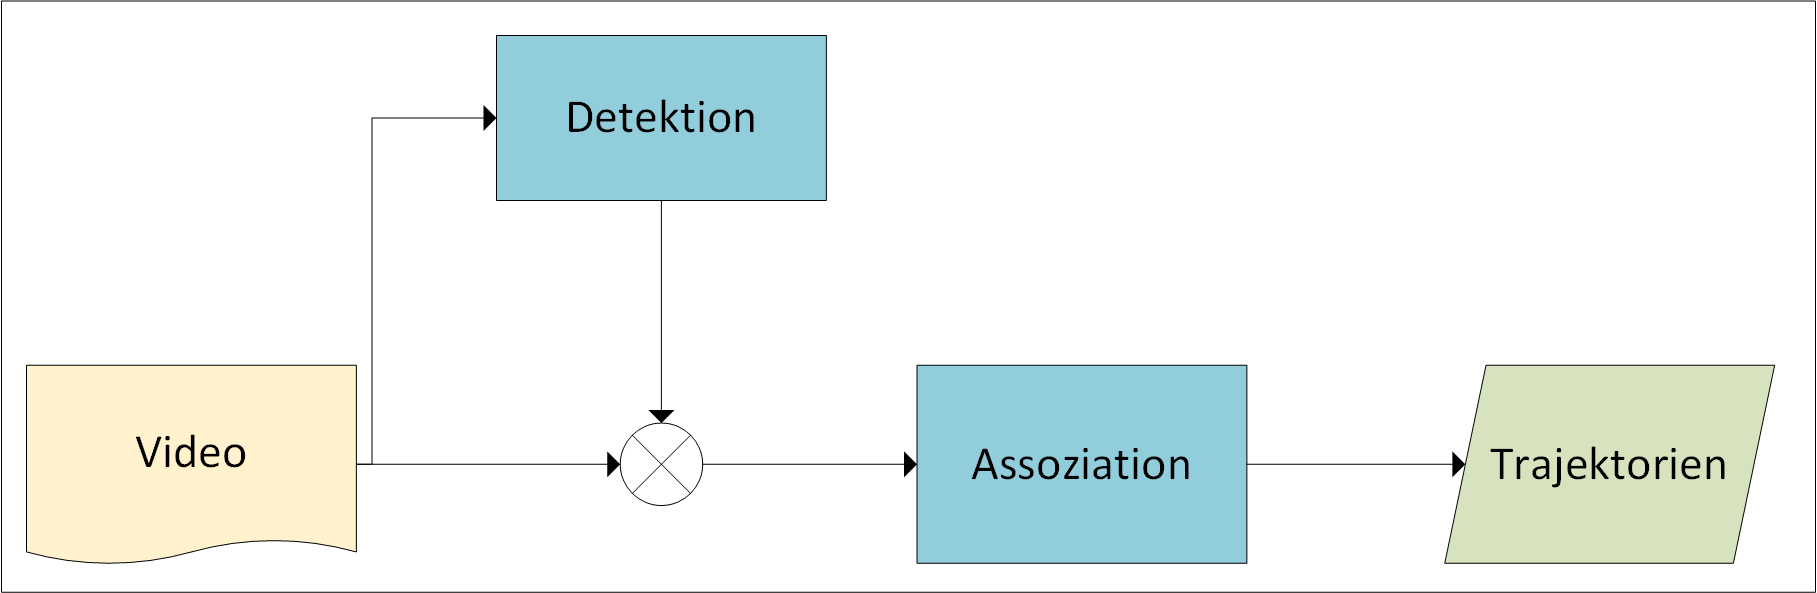
\includegraphics[width=1\textwidth]{img/Grafiken/Detektionsbasiertes Tracking.png}
\caption{Aufbau eines \glsdisp{Detektionsbasiertes Tracking}{detetkionsbasierten Tracking} Systems \cite{Luo.2022}.}
\label{fig:DetBasedTrackSys}
\end{figure}


Die Aufgaben, die ein \gls{MOT} System erfüllen muss lassen sich somit unterteilen in \gls{Detektion}, \gls{Lokalisation} und \gls{Assoziation}. Ziel der \gls{Detektion} ist die Erkennung der Objekte im \gls{Frame}. Die \gls{Lokalisation} ist dafür zuständig die Position der der Objekt im \gls{Frame} zu bestimmen. Aufgabe der \gls{Assoziation} ist es die \gls{Detektion}[en] über alle \gls{Frame}[s] zu verknüpfen, so dass sie konstant einem Objekt zugeordnet sind \cite{CLEAR.2008, HOTA}. In der \autoref{fig:DetBasedTrackSys} sind diese Aufgaben mit dargestellt. Im Folgenden wird unterschieden zwischen der \gls{Detektion} als Aufgabe eines \gls{MOT} Systems und einer \gls{Detektion} als Erkanntes Objekt in einem \gls{Frame}. Ist von einem erkannten Objekt die Rede, so umfasst eine \gls{Detektion} die Erkennung, sowie die \glsdisp{Lokalisation}{Positionsbestimmung} des Objektes. \par

Eine \gls{MOT} System \glsdisp{Detektion}{detektiert} und \glsdisp{Lokalisation}{lokalisiert} Objekte mit Rechtecken, welche möglichst eng um das Objekt gelegt werden. Ein solches Rechtecke wird \gls{Bounding Box} genannt. Es bestimmt die Position des Objektes auf einen begrenzen Bereich. Weiter Darstellungsmöglichkeiten einer \gls{Detektion} sind Punkte Segmentierung von Regionen die zu einem Objekt gehören oder 3D \gls{Bounding Box}. Die 2D \gls{Bounding Box} ist jedoch am verbreitetsten \cite{MOT15, HOTA, Luo.2022}. \par 

\subsection{Herausforderungen für Multi-Object Tracking} \label{sec:MOT Herausforderungen}
In der Praxis existieren Herausforderungen, welche \gls{MOT} erschweren. Den Objekten konstante Identitäten zuzuweisen ist kompliziert, wenn Verdeckungen regelmäßig auftreten. Verdeckungen können durch Sichtblockaden verursacht werden, wie z.B. eine Straßenlaterne in einem Fußgänger\glsdisp{Ereignis}{ereignis}. Ebenso können sie Objekte gegenseitig Verdecken. In solchen Fällen kann es schwierig sein die Identitäten der Objekte nicht zu vertauschen. Ebenfalls kann es herausfordernd sein Identitäten konstant zu halten, wenn Objekte den Kamerabereich verlassen und betreten. Manche Ansätze verwenden Informationen über die Bewegung eines Objektes für die  \gls{Assoziation}, wie die Bewegungsrichtung und die Geschwindigkeit. Solche Informationen sind außerhalb des Kamerabereichs jedoch nicht vorhanden, dies erschwert die \gls{Assoziation}. Um eine bessere \gls{Assoziation} zu erreichen, extrahieren manche Ansätze Informationen über das Aussehen ihrer Objekte, um diese Informationen für die \gls{Assoziation} zu verwenden. Menschen tragen Kleidung in unterschiedlichen Farben, sind unterschiedlich groß und haben unterschiedliche Frisuren. Solche Merkmale können verwendet werden. Besitzen die zu \glsdisp{Assoziation}{assoziierenden} Objekte jedoch eine hohe Ähnlichkeit fällt diese Option weg. Sind \gls{Ereignis}[se] zu tracken, welche eine hohe Objektdichte besitzen verschärft sich die Komplexität. Gerade wenn die Objekte eine hohe Ähnlichkeit besitzen können \gls{Assoziation}[sfehler] häufen. 
In solchen Fällen kann die Bildrate der Kamera ein entscheidender Faktor sein, da sich die \gls{Assoziation} vor allem auf auf die Positionsinformation und Bewegungsinformationen stützen muss. Eine erhöhte Bildrate bedeutet eine höhere Abtastung. Dadurch werden Positionsveränderungen und Veränderungen des Bewegungsprofils feiner Aufgelöst. Dies erleichtert die \gls{Assoziation} in diesen Situationen \cite{Luo.2022, Feng.2022}. \par

Die Performance von einem \glsdisp{Detektionsbasiertes Tracking}{detetkionsbasierten Tracking} System hängt vom \gls{Detektion}\glsdisp{Modul}{smodul} ab. Werden Objekte nicht zuverlässig erkannt, kann die \gls{Assoziation} noch so gut sein, die Qualität der \gls{Trajektorie}[n] wird minderwertig sein \cite{Luo.2022}. 


\subsection{Fehlertypen von Multi-Object Tracking Systemen} \label{sec:MOT Fehlertypen}
In \cite{Leichter.2013} werden fünf Fehlertypen beschrieben, welche im \gls{MOT} auftreten. Diese lassen sich unterteilen in \gls{Detektion}[sfehler], \gls{Assoziation}[sfehler] und \gls{Lokalisation}[sfehler]. \par

\textbf{\gls{Detektion}[sfehler]:}
\begin{itemize}
    \item \textit{\gls{FN}}: Eine falsch negative \gls{Detektion} tritt auf, wenn ein \gls{MOT} System ein Objekt, welches in Wirklichkeit da ist, nicht \glsdisp{Detektion}{detektiert}.
    \item \textit{\gls{FP}}: Eine falsch psoitive \gls{Detektion} tritt auf, wenn ein \gls{MOT} System ein Objekt \glsdisp{Detektion}{detektiert}, welches in Wirklichkeit nicht da ist.
\end{itemize}

\textbf{\gls{Assoziation}[sfehler]:}
\begin{itemize}
    \item \textit{\gls{Fragmentation}}: Eine Fragmentation tritt auf, wenn ein Objekt in den vergangenen \gls{Frame}[s] eine \acrshort{ID} \(a\) zugewiesen bekommen hat und im aktuellen \gls{Frame} eine \acrshort{ID} \(b\) erhält. Die korrekte \gls{Trajektorie} des Objektes besteht aus dem Fragment mit der \acrshort{ID} \(a\) und \(b\). Eine Unvollständige \gls{Trajektorie} zählt ebenfalls als Fragmentation. 
    \item \textit{\gls{Merging Fehler}}: Ein Merging Fehler ist das gegenstück zur Fragmentation. Er tritt auf, wenn zwei Objekte, Objekt \(e\) und Objekt \(f\) vom System die gleiche \acrshort{ID} erhalten. Das System hält die beiden Objekte für ein einzelnes Objekt. 
\end{itemize}

\textbf{\gls{Lokalisationsfehler}:}
\begin{itemize}
    \item Bei der \gls{Lokalisation} liegt der Fehler in der Abweichung von der genauen Position des Objekts \cite{Leichter.2013}. \par
\end{itemize}

In der \autoref{fig:ErrorTypesMOT} sind die unterschiedlichen Fehlerarten illustriert. 


\begin{figure}[htb]
 \centering
 \begin{subfigure}[htb]{0.7\textwidth}
     \centering
     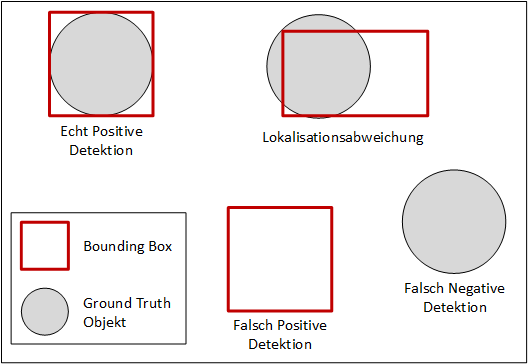
\includegraphics[width=\textwidth]{img/Grafiken/MOT Fehlerarten Detektionen.png}
     \caption{Detektionsfehlerarten}
 \end{subfigure}
 \hfill
 \begin{subfigure}[htb]{0.7\textwidth}
     \centering
     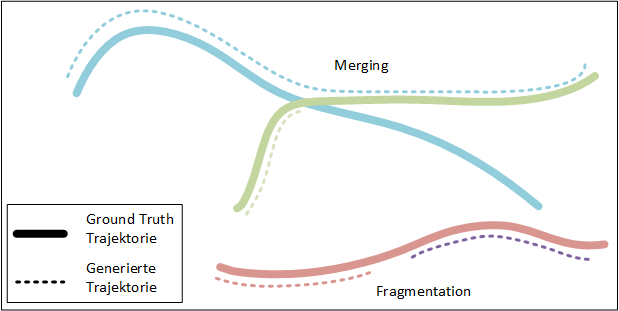
\includegraphics[width=\textwidth]{img/Grafiken/MOT Fehlerarten Assoziation.png}
     \caption{Assoziationsfehlerarten}
 \end{subfigure}
    \caption{Fehlerarten eines \gls{MOT} Systems \cite{Leichter.2013}.}
    \label{fig:ErrorTypesMOT}
\end{figure}


\textbf{Weitere Fehler:}
Gerade ältere Literatur definiert Fehlertypen im \gls{MOT} anders. In der neueren Literatur sind jedoch die oberen Fehlertypen etabliert.

\begin{itemize}
    \item \textit{(\gls{IDSW}}: Ein \gls{IDSW} hat parallelen zur Fragmentation. Er tritt auf, wenn sich die \gls{ID} eines Objektes ändert, obwohl sie konstant bleiben sollte. Dabei berücksichtigt eine \gls{IDSW} jedoch keine unvollständigen \gls{Trajektorie}. Wird eine \gls{Trajektorie} abgebrochen, obwohl sich das Objekt weiter im \gls{Ereignis} befindet gibt es keine \acrshort{ID} die sich ändern kann \cite{CLEAR.2008, HOTA, IDF1}.
\end{itemize}

\subsection{Verarbeitungsverfahren von Multi-Object Tracking Systemen} \label{sec:MOT Verarbeitungsverfahren}
Bei \gls{MOT} Systemen existieren zwei Verarbeitungsverfahren zwischen denen unterschieden wird: Das \gls{Offline Tracking} und das \gls{Online Tracking}. Beim \gls{Online Tracking} werden die \gls{Frame}[s] eines Videos sequentiell verarbeitet. Das bedeutet für die \gls{Assoziation} im \gls{Frame} des Zeitpunktes \(t=N\) stehen nur die \gls{Detektion}[en] der Zeitpunkte \(t \leq N\)  zur Verfügung. Zukünftige \gls{Detektion}[en] werden nicht Berücksichtigt \cite{Luo.2022}. Aus diesem Grund eignen sich \gls{Online Tracking} Systeme besonders für Echtzeitanwendungen \cite{Bewley.2016}. \gls{Offline Tracking} Systeme verarbeiten die \gls{Frame}[s] gebündelt. Bei der \gls{Assoziation} stehen alle \gls{Detektion}[en] aus allen \gls{Frame}[s] zur Verfügung \cite{Luo.2022}. Dadurch ist es möglich, dass mittels globaler Optimierung der \gls{Assoziation} über die \gls{Frame}[s] qualitativ besonders gute \gls{Trajektorie}[n] generiert werden können. Für eine Echtzeitverarbeitung eignen sich \gls{Offline Tracking} Systeme nicht \cite{Luo.2022}. \par